\chapter{Other low-energy physics with P-type point contact detectors}

		
	\section{Other dark matter: heavy axions}
	\label{sec:CalcLimitsOnHeavyAxions}		
		


	\subsection{Heavy axion signal}
	\label{sec:CalcLimitsOnHeavyAxionSignal}		

		\begin{figure}
			\centering
			%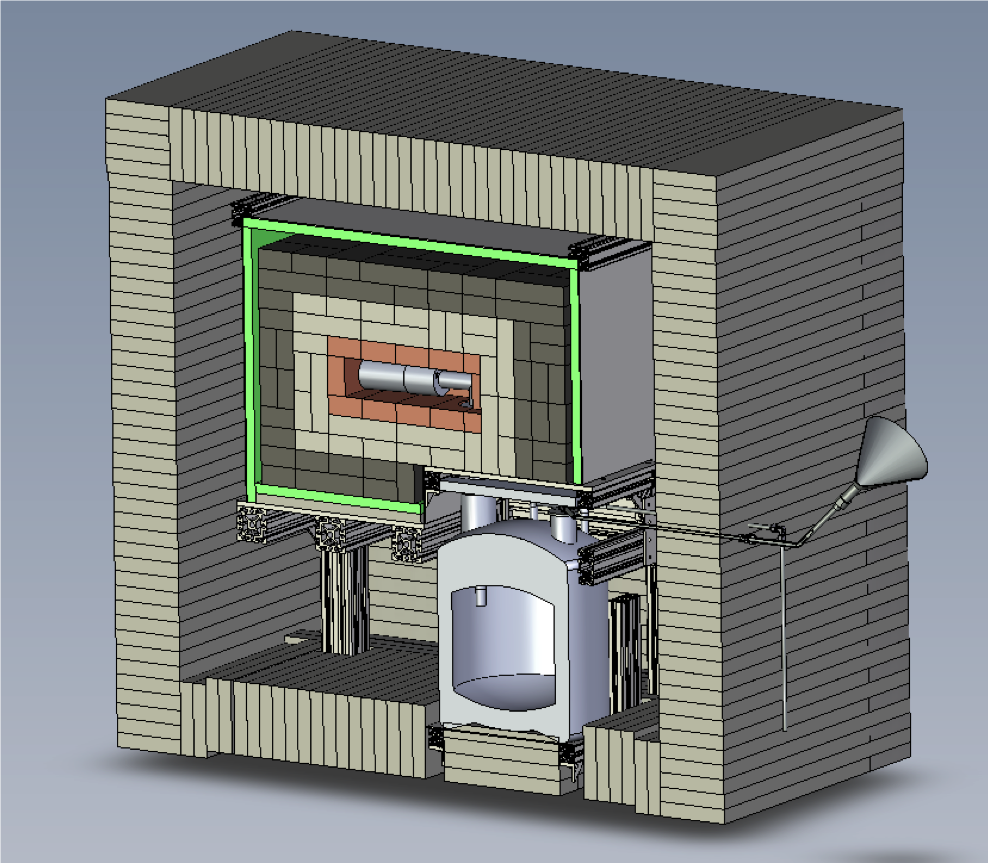
\includegraphics[width=0.9\textwidth]{PPC2DesignSchematicAll}
			\caption{Possible Heavy Axion Dark Matter signal.}
			\label{fig:HeavyAxionSignal}
		\end{figure}

	\subsection{Heavy axion limits}
	\label{sec:CalcLimitsOnHeavyAxionLimits}		
				
		\begin{figure}
			\centering
			%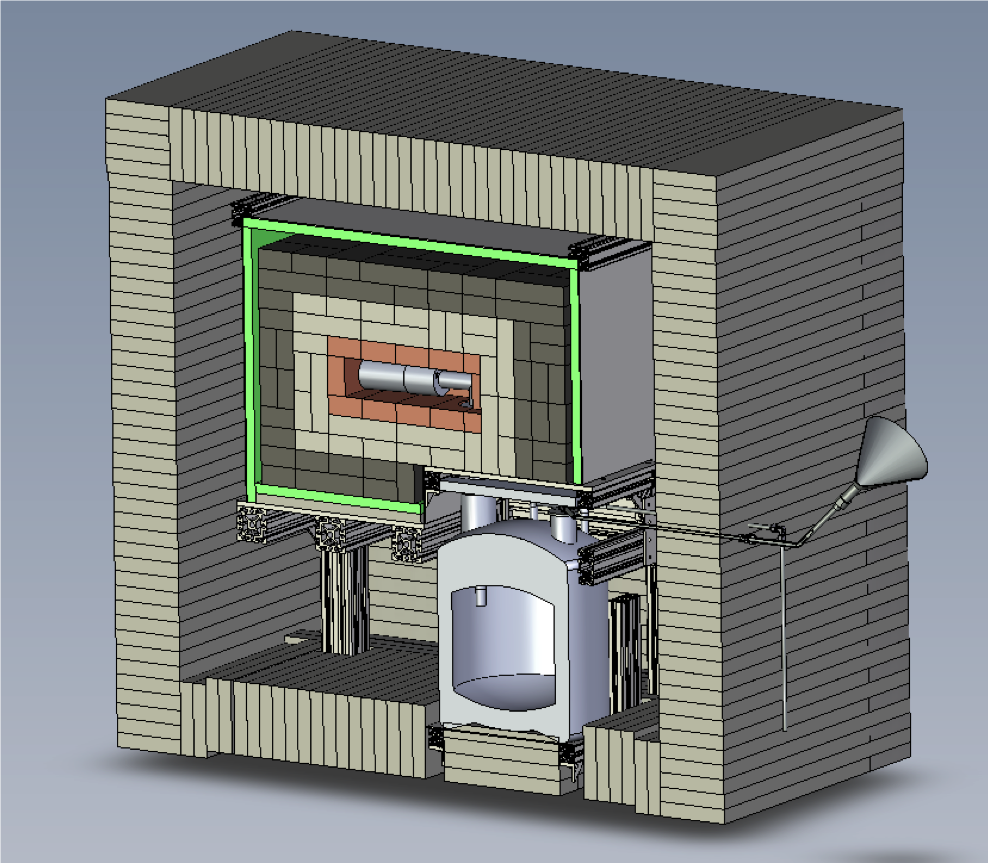
\includegraphics[width=0.9\textwidth]{PPC2DesignSchematicAll}
			\caption{Limits on heavy axions.}
			\label{fig:HeavyAxionSignal}
		\end{figure}
		
							
	\section{Sensitivity of the \MJ~\minmod~to a Dark Matter signal}
	\label{sec:MJSensitivity}
	
		\subsection{Low-energy background model}
		\label{sec:MJLowEnergyBackgroundModel}
		
		\subsection{WIMPs}
		\label{sec:MJSensitivityToWIMP}
		
			\begin{figure}
				\centering
				%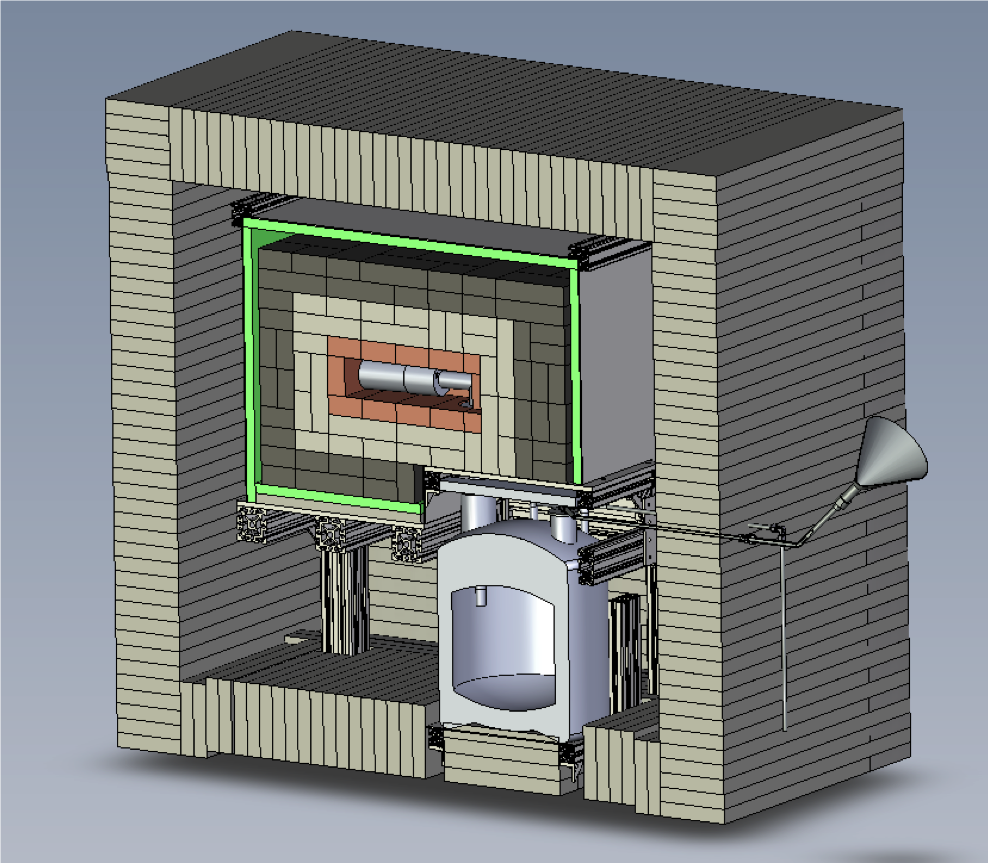
\includegraphics[width=0.9\textwidth]{PPC2DesignSchematicAll}
				\caption{\MJ~\minmod~sensitivity to a WIMP signal.}
				\label{fig:MJSensitivityToWIMP}
			\end{figure}		
			
		\subsection{Heavy axions}
		\label{sec:MJSensitivityToAxions}
		
			\begin{figure}
				\centering
				%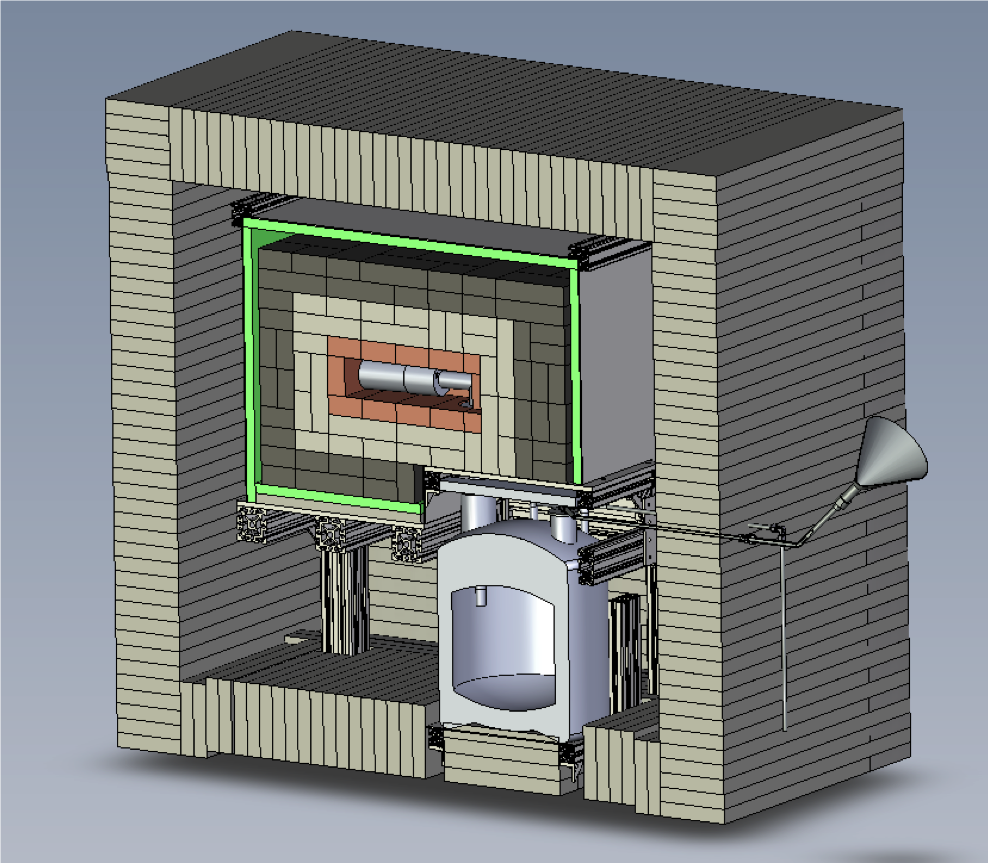
\includegraphics[width=0.9\textwidth]{PPC2DesignSchematicAll}
				\caption{\MJ~\minmod~sensitivity to a Heavy Axion signal.}
				\label{fig:MJSensitivityToHeavyAxions}
			\end{figure}		
			
		%\subsection{Generic Oscillation Signal}
		%\label{sec:MJSensitivityToGenOsc}
		
			%\begin{figure}
			%	\centering
			%	%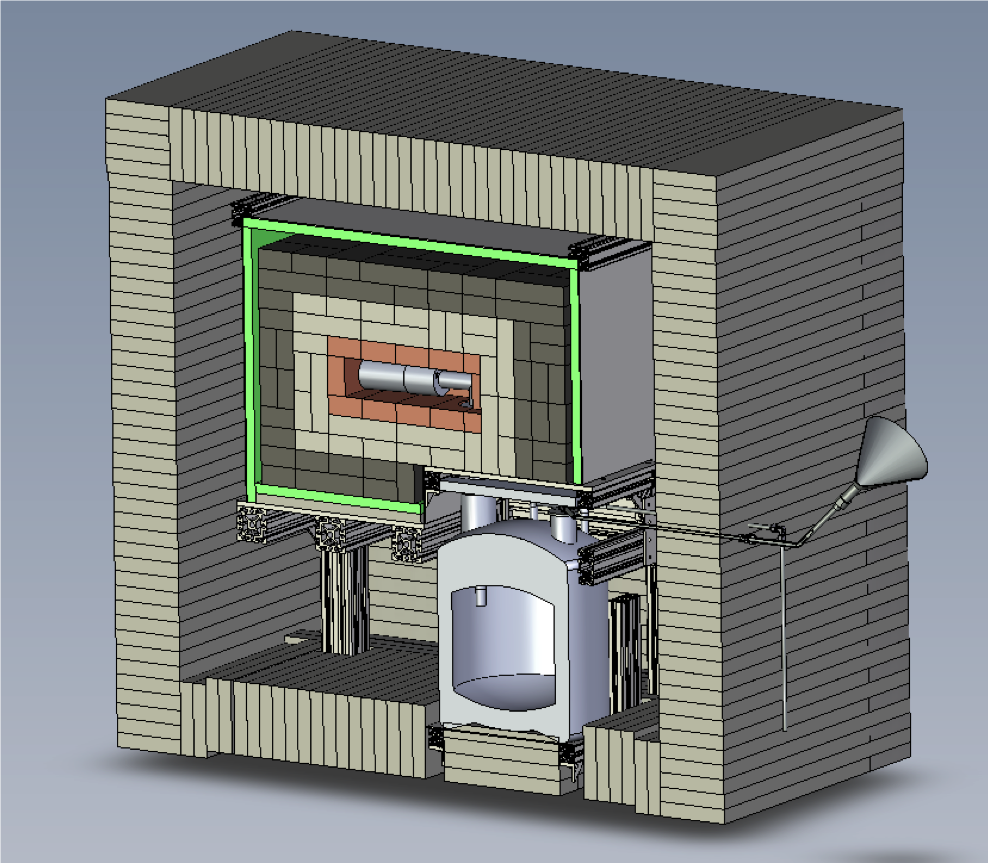
\includegraphics[width=0.9\textwidth]{PPC2DesignSchematicAll}
			%	\caption{\MJ~\minmod~sensitivity to a generic oscillation signal.}
			%	\label{fig:MJSensitivityToGenOscSignal}
			%\end{figure}					

	\section{Conclusions}
	\label{sec:OtherLowEnergyConclusions}	